
We perform our evaluation on an Intel Core 2 dual-processor CPU system
equipped with 16GB of RAM. Each processor is a 4-core 64-bit Xeon
running at 2.33GHZ with a 4MB L2 cache.  The operating system is
CentOS 5.5 (unmodified), running with Linux kernel version
2.6.18-194.17.1.el5. The glibc version is 2.5. Benchmarks were built as 32-bit executables with version
2.6 of the LLVM compiler.

\subsection{Methodology}

We evaluate the performance and scalability of \dthreads{} versus
CoreDet and \pthreads{} across the PARSEC~\cite{parsec} and
Phoenix~\cite{phoenix-hpca} benchmark suites.  We do not include
results for \texttt{bodytrack}, \texttt{fluidanimate}, \texttt{x.264},
\texttt{facesim}, \texttt{vips}, and \texttt{raytrace} benchmarks from PARSEC, 
since they do not currently work with \dthreads{} (note that many of
these also do not work for CoreDet).

In order to compare performance directly against CoreDet, which relies
on the LLVM infrastructure~\cite{LLVM:CGO04}, all benchmarks are
compiled with the LLVM compiler at the ``-O3'' optimization
level~\cite{LLVM:CGO04}. Each benchmark is executed ten
times on a quiescent machine. To reduce the effect of outliers, the
lowest and highest execution times for each benchmark are discarded,
so each result is the average of the remaining eight runs.

\textbf{Tuning CoreDet: } 
The performance of CoreDet~\cite{Bergan:2010:CCR:1736020.1736029} is
extremely sensitive to three parameters: the granularity for the
ownership table (in bytes), the quantum size (in number of
instructions retired), and the choice between full and
reduced serial mode. We performed an extensive search of the parameter
space to find the one that yielded the lowest average normalized
runtimes (using six possible granularities and eight possible quanta for each
benchmark), and found that the best settings on our system were
64-byte granularity and a quantum size of 100,000 instructions, in
full serial mode.

\textbf{Unsupported Benchmarks: }
We were unable to evaluate \dthreads{} on seven of the PARSEC benchmarks: \texttt{vips} and \texttt{raytrace} would not build as 32-bit executables; 
\texttt{bodytrack}, \texttt{facesim}, and \texttt{x264} depend on sharing of stack variables; \texttt{fluidanimate} uses ad-hoc synchronization, so it will not run without modifications; and \texttt{freqmine} does not use \pthreads{}.

For all scalability experiments, we logically disable CPUs using
Linux's CPU hotplug mechanism, which allows us to disable or enable
individual CPUs by writing ``0'' (or ``1'') to a special pseudo-file
(\texttt{/sys/devices/system/cpu/cpuN/online}).

\subsection{Determinism}

We first experimentally verify \dthreads{}' ability to ensure
determinism by executing the \emph{racey} determinism
tester~\cite{1508256}. This stress test is extremely sensitive to
memory-level non-determinism. \dthreads{} reports the same results for
2,000 runs.  We also compared the schedules and outputs of all benchmarks used
to ensure that every execution is identical.

\subsection{Performance}
\label{sec:performance}

We next compare the performance of \dthreads{} to CoreDet
and \pthreads{}. Figure~\ref{fig:performance} presents these results
graphically (normalized to \pthreads{}).

% Table~\ref{tbl:benchmarks} provides detailed numbers.

\dthreads{} outperforms CoreDet on 12 out
of 14 benchmarks (between 14\% and $11.2\times$ faster); 
for 8 benchmarks, \dthreads{} matches or outperforms \pthreads{}.  \dthreads{} results in good performance for several reasons:

\begin{itemize}
	\item Process invocation is only slightly more expensive than thread
	creation.  This is because both rely on the \texttt{clone} system call.
	Copy-on-write semantics allow process creation without expensive copying.

	\item Context switches between processes are more expensive than for threads 
	because of the required TLB shootdown.  The number of context switches was minimized by running on a quiescent system with the number of threads matched to the number of cores whenever possible.

	\item \dthreads{} incurs no read overhead and very
	low write overhead (one page fault per written page), but commits are 	expensive.  Most of our benchmarks (and many real applications) result in 
	small, infrequent commits.

	\item \dthreads{} isolates updates in separate processes, which can improve performance by eliminating false sharing.  Because threads actually execute in different address spaces, there is no coherence traffice between synchronization points.
\end{itemize}

By eliminating catastrophic false sharing, \dthreads{} dramatically
improves the performance of the \texttt{linear\_regression} benchmark,
running $7\times$ faster than \pthreads{} and $11.2\times$ faster than
CoreDet. The \texttt{string\_match} benchmark exhibits a similar, if
less dramatic, false sharing problem: with \dthreads{}, it runs almost
$40\%$ faster than \pthreads{} and $9.2\times$ faster than CoreDet. Two
benchmarks also run faster with \dthreads{} than with \pthreads{}
(\texttt{histogram}, $2\times$ and \texttt{swaptions}, $5\%$;
respectively $8.5\times$ and $8.9\times$ faster than with CoreDet). We
believe but have not yet verified that the reason is false sharing.

For some benchmarks, \dthreads{} incurs modest overhead. For example,
unlike most benchmarks examined here, which create long-lived threads,
the
\texttt{kmeans} benchmark creates and destroys over 1,000 threads over the course of one run.
While Linux processes are relatively lightweight, creating and tearing
down a process is still more expensive than the same operation for
threads, accounting for a $5\%$ performance degradation of \dthreads{}
over \pthreads{} (though it runs $4.9\times$ faster than CoreDet).

\dthreads{} runs substantially slower than \pthreads{} for 4 of the 14
benchmarks examined here. The \texttt{ferret} benchmark relies on an
external library to analyze image files during the first stage in its
pipelined execution model; this library makes intensive (and in the
case of \dthreads{}, unnecessary) use of locks. Lock acquisition and
release in \dthreads{} imposes higher overhead than
ordinary \pthreads{} mutex operations. More importantly in this case,
the intensive use of locks in one stage forces \dthreads{} to
effectively serialize the other stages in the pipeline, which must
repeatedly wait on these locks to enforce a deterministic lock
acquisition order. The other three benchmarks
(\texttt{canneal}, \texttt{dedup}, and \texttt{reverse\_index}) modify
a large number of pages. With \dthreads{}, each page modification
triggers a segmentation violation, a system call to change memory
protection, the creation of a private copy of the page, and a
subsequent copy into the shared space on commit. We note that CoreDet
also substantially degrades performance for these benchmarks, so much
of this slowdown may be inherent to any deterministic runtime system.

\subsection{Scalability}
\label{sec:scalability}

% CCC: Moved scalability figure to evaluation.tex to place on proper page

To measure the scalability cost of running \dthreads{}, we ran our
benchmark suite (excluding \texttt{canneal}) on the same machine with
eight cores, four corse, and just two cores enabled.  Whenever possible
without source code modifications, the number of threads was matched
to the number of CPUs enabled.  We have found that \dthreads{} scales
at least as well as \pthreads{} for 9 of 13 benchmarks, and scales as
well or better than CoreDet for all but one benchmark
where \dthreads{} outperforms CoreDet by $3.5\times$.  Detailed results of this
experiment are presented in Figure~\ref{fig:scalability} and discussed
below.

The \texttt{canneal} benchmark was excluded from the scalability experiment because it matches the workload to the number of threads, making
the comparison between different numbers of threads invalid.  \dthreads{}
hurts scalability relative to \pthreads{} for the \texttt{kmeans}, \texttt{word\_count}, \texttt{dedup}, and \texttt{streamcluster} benchmarks,
although only marginally in most cases.  In all of these cases, \dthreads{} scales better than CoreDet.

\dthreads{} is able to match the scalability of \pthreads{} for three
benchmarks: \texttt{matrix\_multiply}, \texttt{pca},
and \texttt{blackscholes}.  With \dthreads{}, scalability
actually \emph{improves} over \pthreads{} for 6 out of 13
benchmarks.  This is because \dthreads{} prevents false sharing, avoiding 
unnecessary cache invalidations that normally hurt scalability.

% \textbf{tongping: Should we cite "sheriff" here?}


\subsection{Performance Analysis}

\subsubsection{Benchmark Characteristics}
The data presented in Table~\ref{tbl:characteristics} are obtained
from the executions running on all 8 cores.  Column 2 shows the
percentage of time spent in the serial phase.  In \dthreads{}, all
memory commits and actual synchronization operations are performed in
the serial phase.  The percentage of time spent in the serial phase
thus can affect performance and scalability. Applications with higher
overhead in \dthreads{} often spend a higher percentage of time in the
serial phase, primarily because they modify a large number of pages
that are committed during that phase.

Column 3 shows the number of transactions in each application and
Column 4 provides the average length of each transaction (ms).  Every
synchronization operation, including locks, condition variables,
barriers, and thread exits demarcate transaction boundaries
in \dthreads{}.  For
example, \texttt{reverse\_index}, \texttt{dedup}, \texttt{ferret}
and \texttt{streamcluster} perform numerous transactions whose
execution time is less than 1ms, imposing a performance penalty for
these applications.  Benchmarks with longer (or fewer) transactions run
almost the same speed as or faster than \texttt{pthreads},
including \texttt{histogram} or \texttt{pca}.  In \dthreads{}, longer
transactions amortize the overhead of memory protection and copying.

Column 5 provides more detail on the costs associated with
memory updates (the number and total volume of dirtied pages). From
the table, it becomes clear why \texttt{canneal} (the most notable
outlier) runs much slower with \dthreads{} than with \pthreads{}. This benchmark
updates over 3 million pages, leading to the creation of
private copies, protection faults, and commits to the shared memory
space. Copying alone is quite expensive: we found that copying one
gigabyte of memory takes approximately 0.8 seconds when
using \texttt{memcpy}, so for \texttt{canneal}, copying overhead alone
accounts for at least 20 seconds of time spent in \dthreads{} (out of
a total execution time of 39 seconds).

\textbf{Conclusion: }
For the few benchmarks that perform large numbers of short-lived transactions, modify a large number of pages per-transaction, or both, \dthreads{} can result in substantial overhead.  Most benchmarks examined here run fewer, longer-running transactions with a modest number of modified pages.  For these applications, overhead is amortized.  With the side-effect of eliminating false sharing, \dthreads{} can sometimes even outperform \pthreads{}.

\begin{table}[!t]
\centering
% \footnotesize
\begin{tabular}{l|rrrr}
&
{\bf  Serial} &
\multicolumn{2}{c}{\bf  Transactions} &
%{\bf  Trans.} &
%{\bf  Trans.} &
{\bf  Dirtied}
\\
{\bf  Benchmark} &
{\bf  (\% time)} &
{\bf  Count} &
{\bf  Time (ms)} &
{\bf  Pages}\\
%\hline
%\multicolumn{6}{|c|}{\emph{Phoenix}} \\
\hline
 \textbf{histogram} &  0 &  23 &  15.47 &  29\\
 \textbf{kmeans} &  0 &  3929 &  3.82 &  9466\\
 \textbf{linear\_reg.} &  0 &  24 &  23.92 &  17\\
 \textbf{matrix\_mult.} &  0 &  24 &  841.2 &  3945\\
 \textbf{pca} &  0 &  48 &  443 &  11471\\
 \textbf{reverseindex} &  17\% &  61009 &  1.04 &  451876\\
 \textbf{string\_match} &  0 &  24 &  82 &  41\\
 \textbf{word\_count} &  1\% &  90 &  26.5 &  5261\\
%\hline
%\multicolumn{6}{|c|}{\emph{PARSEC}} \\
%\hline
 \textbf{blackscholes} &  0 &  24 &  386.9 &  991\\
 \textbf{canneal} &  26.4\% &  1062 &  43 &  3606413\\
 \textbf{dedup} &  31\% &  45689 &  0.1 &  356589\\
 \textbf{ferret} &  12.3\% &  11282 &  1.49 &  147027 \\
 \textbf{streamcluster} &  18.4\% &  130001 &  0.04 &  131992\\
 \textbf{swaptions} &  0 &  24 &  163 &  867\\
% \hline
\end{tabular}
\caption{Benchmark characteristics.\label{tbl:characteristics}}
\end{table}

\subsubsection{Performance Impact Analysis}
\label{sec:investigation}
To understand the performance impact of \dthreads{}, we re-ran the benchmark suite on two individual components of \dthreads{}: deterministic synchronization and memory protection.

\textbf{Sync-only:}
This configuration enforces only a deterministic synchronization order.  Threads have direct access to shared memory with no isolation.  Overhead from this component is largely due to load imbalance from the deterministic scheduler.

\textbf{Prot-only:}
This configuration runs threads in isolation, with commits at synchronization points.  The synchronization and commit order is not controlled by \dthreads{}.  This configuration eliminates false sharing, but also introduces isolation and commit overhead.  The lazy twin creation and single-threaded execution optimizations are disabled here because they are unsafe without deterministic synchronization.

\begin{figure*}[!t]
{\centering
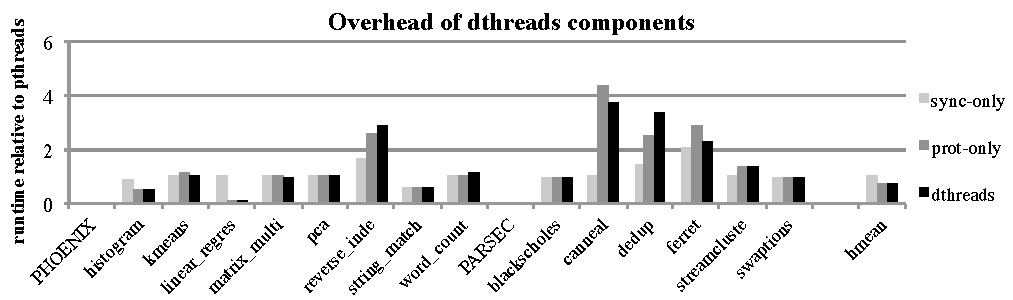
\includegraphics{fig/perfeffect}
\caption{
	Normalized execution time with respect to \pthreads{} (lower is better) for three configurations.  The \emph{sync-only} and \emph{prot-only} configurations are described in Section~\ref{sec:investigation}.
	\label{fig:perfanalysis}}
}
\end{figure*}

The results of this experiment are presented in Figure~\ref{fig:perfanalysis} and discussed below.

\begin{itemize}
	\item
		The \texttt{reverse\_index}, \texttt{dedup}, and \texttt{ferret} benchmarks show significant load imbalance with the {\em sync-only} configuration.  Additionally, these benchmarks have high overhead from the {\em prot-only} configuration because of a large number of transactions.
	
	\item
		Both \texttt{string\_match} and \texttt{histogram} run faster with the {\em sync-only} configuration.  The reason for this is not obvious, but may be due to the per-thread allocator.
	
	\item
		Memory isolation in the {\em prot-only} configuration eliminates false sharing, which resulted in speedups for \texttt{histogram}, \texttt{linear\_regression}, and \texttt{swaptions}.

	\item
		Normally, the performance of \dthreads{} is not better than the {\em prot-only} configuration.  However, both \texttt{ferret} and \texttt{canneal} run faster with deterministic synchronization enabled.  Both benchmarks benefit from optimizations described in Section~\ref{sec:dthreads-optimizations} that are only safe with deterministic synchronization enabled.  \texttt{ferret} benefits from the single threaded execution optimization, and \texttt{canneal} sees performance gains due to the shared twin page optimization.

% CCC: I'm not sure I understand this last comment.  Commenting out for the camera ready draft:
% The reason for \texttt{canneal} is that \dthreads{} simply use a common twin for all threads thus greately reduce the number of twin pages.  

\end{itemize}

% The memory overhead of \dthreads{} includes memory
%protection system calls overhead, memory trap overhead and memory
%commit overhead.  Memory overhead of \dthreads{} are based on page
%granularity, capturing those dirty pages using page protection,
%tracking modifications of one thread by diffing private pages with
%twin pages and committing changes to the shared mapping in the end.

\punt{
\begin{table*}[!t]
\centering
\begin{tabular}{l|rrr|rr|l}
{\bf \small Benchmark} & {\bf \small CoreDet} & {\bf \small \dthreads{}} & {\bf \small \pthreads{}} & $\frac{\mbox{\bf \small CoreDet}}{\mbox{\bf \small \pthreads{}}}$ & $\frac{\mbox{\small \bf \dthreads{}}}{\mbox{\small \bf \pthreads{}}}$ & {\bf \small Input} \\

\hline
{\bf \small histogram} & 0.97 & 0.35 & 0.73 & $1.32\times$ & $0.48\times$ & {\it \small large.bmp} \\
{\bf \small kmeans} & 68.41 & 15.02 & 13.16 & $5.20\times$ & $1.14\times$ & {\it \small -d 3 -c 1000 -p 100000 -s 1000} \\ 
{\bf \small linear\_regression} & 6.42 & 0.57 & 4.11  & $1.56\times$ & $0.14\times$ & {\it \small key\_file\_500MB.txt} \\
{\bf \small matrix\_multiply} & 31.68 & 19.28 & 19.32  & $1.63\times$ & $0.99\times$ & {\it \small 2000 2000 } \\
{\bf \small pca} & 39.24 & 21.14  & 20.49 & $1.92\times$ & $1.03\times$ & {\it \small -r 4000 -c 4000 -s 100 } \\
{\bf \small reverse\_index} & 7.85 & 6.53 & 2.06 & $3.81\times$ & $3.17\times$ & {\it \small datafiles} \\
{\bf \small string\_match} & 18.31 & 1.97 &  3.19 & $5.74\times$ & $0.62\times$ & {\it \small key\_file\_500MB.txt} \\
{\bf \small word\_count} & 17.17 & 2.37 & 2.17 & $7.91\times$ & $1.09\times$ & {\it \small word\_100MB.txt} \\
{\bf \small blackscholes} & 10.49 & 9.30 & 9.47 & $1.11\times$ & $0.98\times$ & {\it \small 8 in\_1M.txt prices.txt} \\
{\bf \small canneal} & 14.74 & 39.82  & 10.41 & $1.42\times$ & $3.83\times$ &  {\it \small 7 15000 2000 400000.nets 128} \\
{\bf \small dedup} & 3.38 & 5.39 & 1.45 & $2.33\times$ & $3.72\times$ & {\it \small -c -p -f -t 2 -i media.dat output.txt} \\
{\bf \small ferret} & 21.89 & 16.95 & 7.02 & $3.11\times$ & $2.41\times$ & {\it \small corel lsh queries 10 20 1 output.txt} \\
{\bf \small streamcluster} & 14.33 & 4.61 & 2.74  & $5.23\times$ & $1.68\times$ &  {\it \small 10 20 128 16384 16384 1000 none output.txt 8} \\
{\bf \small swaptions} & 35.21 & 3.88 & 4.18  & $8.42\times$ & $0.93\times$ & {\it \small -ns 128 -sm 50000 -nt 8} \\
% was dthreads, pthreads, coredet
%{\bf \small histogram} & 0.35 & 0.73 & 0.97 & {\bf \small large.bmp} \\
%{\bf \small kmeans} & 15.02 & 13.16 & 68.41 & {\bf \small -d 3 -c 1000 -p 100000 -s 1000} \\ 
%{\bf \small linear\_regression} & 0.57 & 4.11 & 6.42 &  {\bf \small key\_file\_500MB.txt} \\
%{\bf \small matrix\_multiply} & 19.28 & 19.32 & 31.68 & {\bf \small 2000 2000 } \\
%{\bf \small pca} & 21.14 & 20.49 & 39.24 & {\bf \small -r 4000 -c 4000 -s 100 } \\
%{\bf \small reverse\_index} & 6.53 & 2.06 & 7.85 & {\bf \small datafiles} \\
%{\bf \small string\_match} & 1.97 & 3.19 & 18.31 & {\bf \small key\_file\_500MB.txt} \\
%{\bf \small word\_count} & 2.37 & 2.17 & 17.17 & {\bf \small word\_100MB.txt} \\
%{\bf \small blackscholes} & 9.30 & 9.47 & 10.49 & {\bf \small 8 in\_1M.txt prices.txt} \\
%{\bf \small canneal} & 39.82 & 10.41 & 14.74 & {\bf \small 7 15000 2000 400000.nets 128} \\
%{\bf \small dedup} & 5.39 & 1.45 & 3.38 & {\bf \small -c -p -f -t 2 -i media.dat output.txt} \\
%{\bf \small ferret} & 26.86 & 7.02 & 21.89 & {\bf \small corel lsh queries 10 20 1 output.txt} \\
%{\bf \small streamcluster} & 4.61 & 2.74 & 14.33 & {\bf \small 10 20 128 16384 16384 1000 none output.txt 8} \\
%{\bf \small swaptions} & 3.88 & 4.18 & 35.21 & {\bf \small -ns 128 -sm 50000 -nt 8} \\
\hline
\end{tabular}
\caption{Benchmarks: execution time (in seconds) and input parameters.\label{tbl:benchmarks}}
\end{table*}
}
